\vspace{10pt}

{\centering\subsection*{吴才俊:游十六潭公园}}

\addcontentsline{toc}{subsection}{吴才俊:游十六潭公园}

\renewcommand{\leftmark}{吴才俊:游十六潭公园}

\begin{figure}[htbp]

\centering

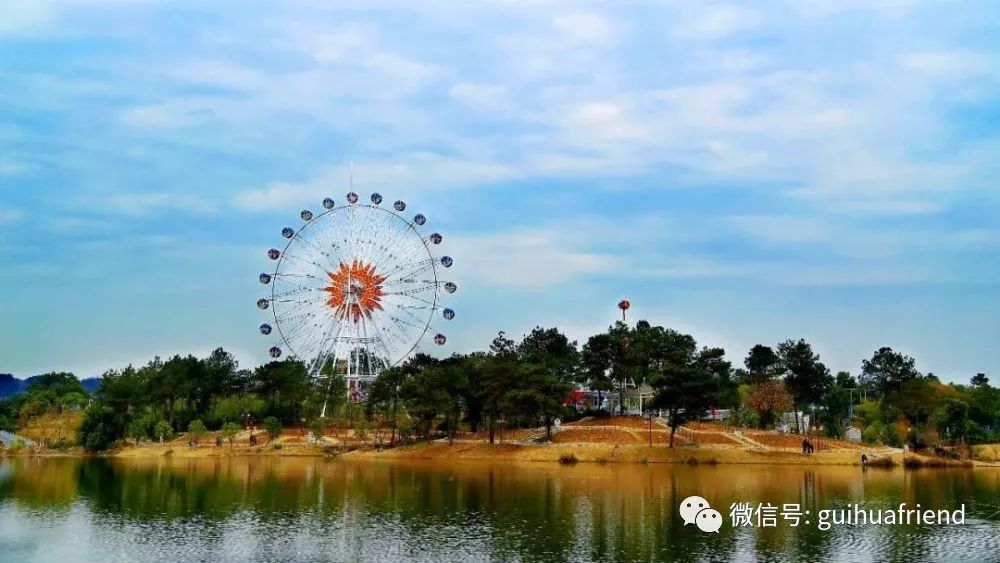
\includegraphics[width = .5\textwidth]{./ch/21.jpg}

\end{figure}





暑假,我和妈妈一起去十六潭公园游玩。

为什么叫十六谭公园呢?因为那里有16个大小不一的水潭,其中最大的水潭是最美的,在水潭的岸上,长着高大挺拔的大树,树被倒映在河中,河中还有几只水鸭子,在水面上时不时把头扎进水里觅食,一群群鱼儿在水下嬉戏。

接下来我们去了十六潭公园里的游乐场玩。刚进入游乐场,就看见了入口处的大石像。

在游乐园中有惊险刺激的大摆锤,旋转飞椅和摩天轮,还有休闲的旋转木马和碰碰车,最让我难忘的是海盗船。

那一次我坐海盗船被吓哭了。我们先刷了卡,我上去坐好,系上安全带。当工作人员确认大家都系上安全带后,把开关打开了,船慢慢摇动,然后越来越快,最后船差点在空中翻了一圈,下来的时候我已经泪流满面了。

这就是美丽的十六潭公园,希望你们也来这里游玩。





\vspace{10pt}



作者:四(1)班 吴才俊



指导老师:周瑞





\vspace{10pt}

\hline



